%%%%%%%% ICLR 2027 LATEX SUBMISSION FILE %%%%%%%%%%%%%%%%%
% Official template: https://media.iclr.cc/Conferences/ICLR2027/iclr-2027-style-files.zip
% Template archive SHA256: 0d940dfa9398ae99a18f24a85a8a683f367204b6af6d17d2899e60a67102529e

\documentclass{article}
% Compile with pdfLaTeX to preserve the official ICLR Times Type 1 fonts.
% XeLaTeX/LuaLaTeX use a different font encoding and can trigger font fallback.
\usepackage{iclr2027_conference,times}

% Recommended, but optional, packages for figures and better typesetting:
\usepackage{microtype}
\usepackage{graphicx}
\usepackage{subcaption}
\usepackage{booktabs} % for professional tables

% hyperref makes hyperlinks in the resulting PDF.
\usepackage{hyperref}

% Keep the submission anonymous; uncomment only for a camera-ready version.
% \iclrfinalcopy

\usepackage{amsmath}
\usepackage{amssymb}
\usepackage{mathtools}
\usepackage{amsthm}


% if you use cleveref..
\usepackage[capitalize,noabbrev]{cleveref}

%%%%%%%%%%%%%%%%%%%%%%%%%%%%%%%%
% THEOREMS
%%%%%%%%%%%%%%%%%%%%%%%%%%%%%%%%
\theoremstyle{plain}
\newtheorem{theorem}{Theorem}[section]
\newtheorem{proposition}[theorem]{Proposition}
\newtheorem{lemma}[theorem]{Lemma}
\newtheorem{corollary}[theorem]{Corollary}
\theoremstyle{definition}
\newtheorem{definition}[theorem]{Definition}
\newtheorem{assumption}[theorem]{Assumption}
\theoremstyle{remark}
\newtheorem{remark}[theorem]{Remark}

% Todonotes is useful during development; simply uncomment the next line
%    and comment out the line below the next line to turn off comments
%\usepackage[disable,textsize=tiny]{todonotes}
\usepackage[disable,textsize=tiny]{todonotes}

% add packages
\usepackage{amsmath}
\usepackage{amssymb}
\usepackage{amsthm}
\usepackage{enumitem}
\usepackage{algpseudocode}
\usepackage{booktabs}       % For professional tables
\usepackage{subcaption}
\usepackage{nameref}      % For \nameref
\usepackage{algorithm}
\usepackage{multirow}       % For tables in appendix
\usepackage{url}            % For \url
\usepackage{hyperref}       % For \href
\usepackage{cleveref}
\usepackage{adjustbox}

% Separate top and bottom floats with the page body.
\setcounter{topnumber}{1}
\setcounter{bottomnumber}{1}
\setcounter{totalnumber}{2}
\Crefname{equation}{Eq.}{Eqs.}

\newcommand{\ours}{REINFORCE++\,}
\newcommand{\varn}{REINFORCE++\textsubscript{\textit{w/} Baseline}\,}

% Attempt to make hyperref and algorithmic work together better:
% \newcommand{\theHalgorithm}{\arabic{algorithm}}



\title{REINFORCE++: Stabilizing Critic-Free Policy\\Optimization with Global Normalization}

% Original author and affiliation metadata, hidden by the ICLR review style.
\author{%
  Firstname1 Lastname1\textsuperscript{*,1},
  Firstname2 Lastname2\textsuperscript{*,1,2},
  Firstname3 Lastname3\textsuperscript{2} \\
  Firstname4 Lastname4\textsuperscript{3},
  Firstname5 Lastname5\textsuperscript{1},
  Firstname6 Lastname6\textsuperscript{3,1,2} \\
  Firstname7 Lastname7\textsuperscript{2},
  Firstname8 Lastname8\textsuperscript{3},
  Firstname8 Lastname8\textsuperscript{1,2} \\
  \textsuperscript{1}Department of XXX, University of YYY, Location, Country \\
  \textsuperscript{2}Company Name, Location, Country \\
  \textsuperscript{3}School of ZZZ, Institute of WWW, Location, Country \\
  Correspondence to: Firstname1 Lastname1 \texttt{first1.last1@xxx.edu}, \\
  Firstname2 Lastname2 \texttt{first2.last2@www.uk}
}
\hypersetup{
  pdftitle={REINFORCE++: Stabilizing Critic-Free Policy Optimization with Global Normalization},
  pdfauthor={Anonymous Authors},
  pdfkeywords={Machine Learning, Reinforcement Learning, ICLR}
}

\begin{document}

\maketitle

\begin{abstract}
Critic-free reinforcement learning reduces the cost of post-training large language models, but its behavior depends strongly on how rewards are converted into advantages. In group-relative methods, normalizing rewards separately for each prompt couples the update scale to statistics estimated from a small set of responses. We introduce REINFORCE++, a critic-free policy optimization framework that instead normalizes advantages across the rollout batch. The basic variant supports one or more responses per prompt and incorporates a token-level KL penalty into Monte Carlo returns. A second variant, REINFORCE++-Baseline, combines a within-prompt reward baseline with global normalization and a separate KL regularizer. Our analysis characterizes finite-sample normalization and its convergence to population standardization under independent sampling. Experiments cover preference-based alignment, mathematical and logical reasoning, and multi-step tool use. With one response per prompt, REINFORCE++ obtains an Arena-Hard score of 46.7, compared with 46.8 for four-response GRPO. In tool-use experiments, REINFORCE++-Baseline achieves an average score of 24.10, compared with 22.58 for GRPO and 21.85 for PPO. These results support global normalization as a practical design choice for critic-free language-model training.
\end{abstract}

\section{Introduction}

Reinforcement Learning from Human Feedback (RLHF) is a key technique for aligning Large Language Models~(LLMs) with human values and preferences ~\citep{vemprala2023chatgpt,achiam2023gpt, Ouyang2022, shen2024policy,shen2025exploring,hu2024openrlhf}. Despite the emergence of non-RL alternatives like DPO ~\citep{rafailov2023direct}, state-of-the-art applications such as ChatGPT/GPT-4 ~\citep{vemprala2023chatgpt, openai2023gpt4}, Claude ~\citep{anthropic2023introducing}, and Gemini ~\citep{team2023gemini} continue to rely on RL algorithms.

The dominant RL algorithm in this space is Proximal Policy Optimization (PPO) ~\citep{schulman2017proximal}. PPO employs an "Actor-Critic" architecture, where a dedicated critic network is trained to estimate the advantage function (i.e., the extent to which an action yields a higher expected return than the mean). However, this critic network introduces substantial computational overhead and memory requirements, making training prohibitively expensive and limiting large-scale model alignment on small-scale clusters \citep{shao2024deepseekmath}.

To address PPO's efficiency issues, a family of REINFORCE-based methods has emerged without the critic model, including ReMax~\citep{li2023remax}, RLOO~\citep{2024Back}, and GRPO~\citep{shao2024deepseekmath}. These algorithms replace the critic network with an estimator that computes the advantage from multiple responses to the same prompt.

However, this critic-free approach introduces a critical challenge: \textit{advantage estimation}. GRPO uses \textbf{prompt-level (local) normalization}, estimating a baseline and standard deviation from responses to one prompt; RLOO uses a leave-one-out baseline without inherently requiring this scale normalization. These are distinct design choices. First, Appendix~\ref{appendix:proof_GRPO} shows that finite-sample self-normalization differs from population standardization. Second, small groups (e.g., $k=4$ or $k=8$) make the scale sensitive to sampled outcomes. Homogeneous groups provide no centered reward signal, while different reward spreads induce different prompt-specific scales. Finally, these relative comparisons may emphasize fitting individual groups rather than transfer across prompts. Our experiments examine the resulting training dynamics and held-out generalization.

We introduce two distinct variants of this framework, each tailored to a specific use case. \ours is an efficient algorithm with $k \ge 1$. In its $k=1$ configuration (detailed in Algorithm 1), it maximizes prompt diversity for general-domain RLHF. It can also be applied with $k>1$ (Section 4.2), using the same global normalization principle. \varn is a specialized \textit{variant} for complex tasks ($k>1$) that benefits from \textbf{group sampling}. It fixes the flaws of GRPO by first subtracting the \textit{group mean} (for reward reshaping) and then normalizing by the \textit{global standard deviation} (for stability). It also employs a $k_2$ gradient surrogate for separate $\mathrm{KL}$ regularization, as detailed in Appendix~\ref{appendix:kl_design}. In summary, our contributions are as follows:
\begin{itemize}
    \item We provide a theoretical proof that finite-sample local normalization differs from population standardization under explicit sampling assumptions (Appendix~\ref{appendix:proof_GRPO}).
    \item We propose \ours, a critic-free framework centered on Global Advantage Normalization, as a stable, efficient, and theoretically sound alternative.
    % --- MODIFIED: Clarified the two algorithms based on the new k>=1 logic ---
    \item We present two specialized algorithms: We can use \ours when $k \ge 1$ for efficient general RLHF and reasoning, and use \varn when $k>1$ for robust complex agentic tasks.
    % --- END OF MODIFICATION ---
    \item The experiments show that \ours achieves competitive general RLHF scores with shorter responses and stronger held-out reasoning performance. At the same time, \varn outperforms both GRPO and PPO in complex agentic reasoning tasks.
\end{itemize}

\section{Background and Related Work}\label{sec:background}

\begin{figure*}[!ht]
    \centering
    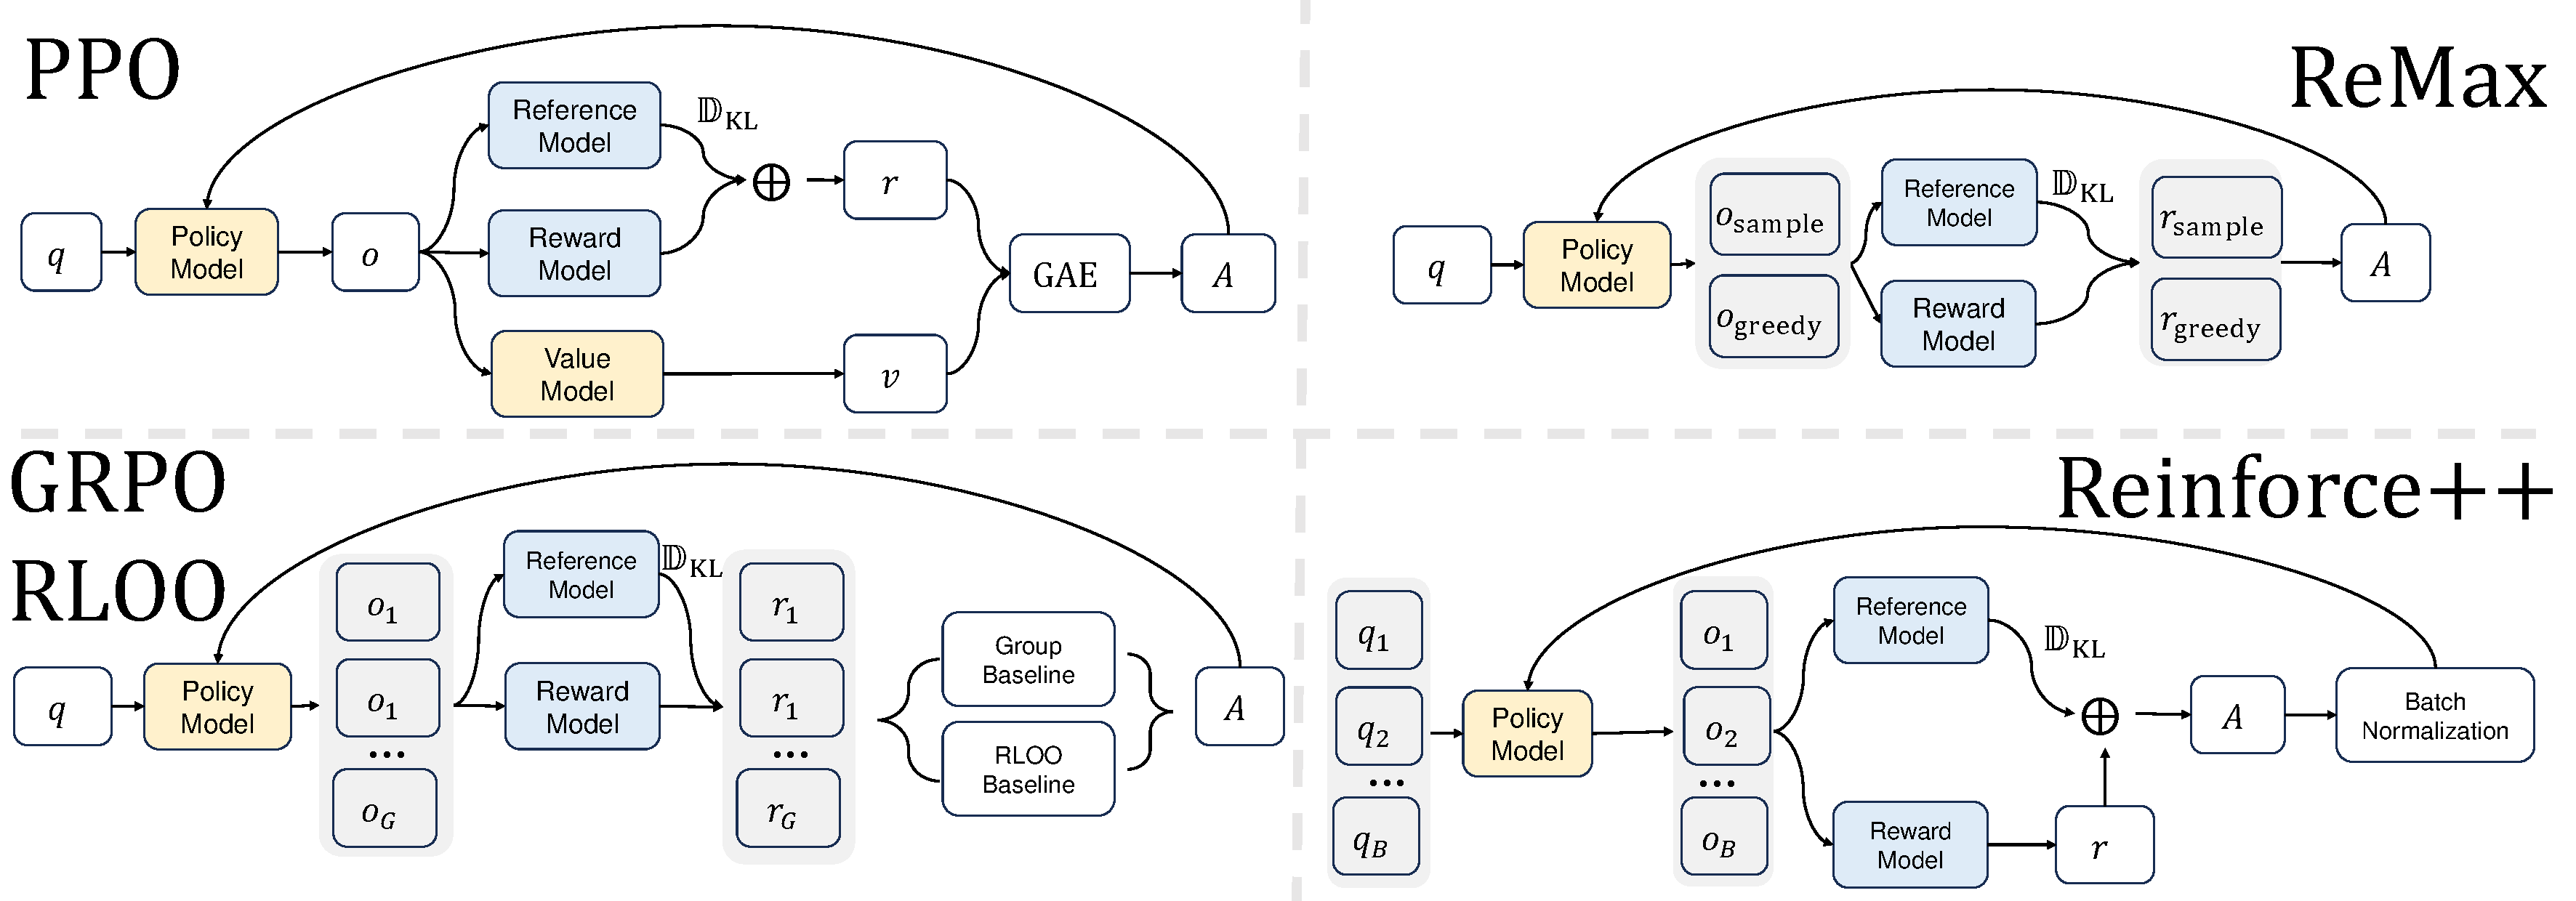
\includegraphics[width=0.85\textwidth]{imgs/re_2.pdf}
    \caption{The comparison of PPO, ReMax, GRPO, RLOO, and \ours. \ours, as shown in the figure, removes the critic model and uses global batch normalization. \varn uses group sampling, similar to GRPO/RLOO, but replaces the local group baseline with a group-mean subtraction followed by global batch normalization.}
    \label{fig:main}
\end{figure*}

\subsection{PPO and Critic-Free RLHF}
PPO optimizes LLMs by maximizing the following surrogate objective:

\begin{equation}\label{eq:ppo}
\begin{adjustbox}{max width=\linewidth}
$
\begin{aligned}
\mathcal{L}_{\text{PPO}}(\theta)
&= \mathbb{E}_{q \sim P(Q),\, o \sim \pi_{\theta_{\text{old}}}(O|q)} \Bigg[
    \frac{1}{|o|} \sum_{t=1}^{|o|}
    \min \Big(
        s_t(\theta) A_t, \\[-2pt]
&\quad \text{clip}(s_t(\theta),\, 1 - \epsilon,\, 1 + \epsilon) A_t
    \Big)
\Bigg]
\end{aligned}
$
\end{adjustbox}
\end{equation}

where $s_t(\theta) = \frac{\pi_{\theta}(o_t | q, o_{<t})}{\pi_{\theta_{\text{old}}}(o_t | q, o_{<t})}$ is the probability ratio. The advantage $A_t$ is typically calculated using Generalized Advantage Estimation~(GAE) \citep{schulman2015high}:
\begin{equation}
    A_{q, o_t} = \sum_{l=0}^{\infty} (\gamma \lambda)^l \delta_{t+l}
\end{equation}
where $\delta_{q, o_t} = r_t + \gamma V(o_{t+1}) - V(o_t)$ is the temporal difference error, and $V(\cdot)$ is the critic network.

Critic-free methods in \Cref{fig:main} remove the critic $V(\cdot)$ and compute the advantage $A_t$ directly from rewards.
\begin{itemize}[leftmargin=*]
    \item \textbf{ReMax} \citep{li2023remax} uses a greedy decoding response $\hat{o}$ as the baseline: $A_{q,o_t} = r(o) - r(\hat{o})$.
    \item \textbf{RLOO} \citep{2024Back} samples $k$ responses and uses the mean of others as the baseline: $A_{q,o_t^{(i)}} = r(o^{(i)}) - \frac{1}{k-1}\sum_{j \neq i} r(o^{(j)})$.
    \item \textbf{GRPO} \citep{shao2024deepseekmath} also samples $k$ responses but normalizes the advantage using the mean and standard deviation of the \textit{local group}:
\end{itemize}
\begin{equation}\label{eq:grpo}
A_{q,o_t^{(i)}} = \frac{r(o^{(i)}) - \text{mean}\bigl(\{r(o^{(j)})\}_{j=1}^{k}\bigr)}{\text{std}\bigl(\{r(o^{(j)})\}_{j=1}^{k}\bigr) + \epsilon}
\end{equation}

\subsection{The Problem with Local Normalization}
The core issue with methods like GRPO lies in \Cref{eq:grpo}. The usage of \textbf{prompt-level (local) normalization} is problematic for three reasons:
\begin{enumerate}
    \item \textbf{Theoretical Bias}: As formally proven in Appendix \Cref{appendix:proof_GRPO}, the estimator is biased. Therefore, the numerator (centered reward) and the denominator (local standard deviation $\text{std}(\cdot)$) are not independent. The denominator's value is correlated with the rewards in the small group, introducing a systematic error in the advantage estimate \citep{mai2025agent}.
    \item \textbf{Practical Instability}: In practice, the group size $k$ is small (e.g., 4 or 8). If all sampled responses for a prompt happen to get similar rewards, the local $\text{std}(\cdot)$ approaches zero, causing the advantage to explode. It results in high variance and unstable training.
    \item \textbf{Task Overfitting}: The policy is rewarded for being "better than other samples from the same prompt," not for being "globally good." It can lead to overfitting on simple prompts where it's easy to generate diverse rewards, while failing to improve on complex prompts.
\end{enumerate}

\section{Method}\label{sec:method}


Our method addresses the instability of critic-free RLHF by replacing biased local normalization with stable global normalization. We propose two variants for different use cases.

\subsection{Global Normalization}

The primary \ours algorithm is designed for general-purpose RLHF. In its $k=1$ configuration, it is designed for maximum efficiency and prompt diversity.

It optimizes the PPO objective in \Cref{eq:ppo} but redefines the advantage $A_{q,o_t}$. We use the standard PPO reward formulation, which incorporates the k1-style KL penalty directly into the reward:
\begin{equation}\label{eq:adv}
A_{q,o_t} = r(o_{1:T},q) - \beta \cdot \sum_{i=t}^{T} \mathrm{KL}(i)
\end{equation}
where $\text{KL}(t) = \log\left(\frac{\pi_{\theta_{\text{old}}}(o_t | q, o_{<t})}{\pi_{ref}(o_t | q, o_{<t})}\right)$.

The key innovation is our normalization strategy. Instead of a non-existent (for $k=1$) or biased local norm, we use Global Advantage Normalization~\citep{andrychowicz2020matters}:
\begin{equation}\label{eq:batch_norm}
A_{q,o_t}^{\text{norm}} = \frac{A_{q,o_t} - \text{mean}\left(A|A \in \mathcal{D}_{\text{batch}}\right)}{\text{std}\left(A|A \in \mathcal{D}_{\text{batch}}\right) + \epsilon}
\end{equation}
The global normalization is the core of \ours. Pooling a large rollout batch (e.g., 1024 responses) replaces separate small-group scales with shared statistics. Under independent sampling, sample moments converge to population values (Appendix~\ref{appendix:proof_GRPO}); this is not a general unbiased-policy-gradient guarantee. Valid token positions exclude padding, and the moments remain fixed during rollout reuse.
The efficient $k=1$ case is detailed in \Cref{algo:main}.


\subsection{Local Baseline}
For more complex tasks, such as multi-step reasoning, sampling multiple responses per prompt ($k > 1$) can be beneficial \citep{yue2025vapo}. To this end, we introduce \varn. This variant combines the benefits of group-sampling with the stability of global normalization. The advantage calculation is a two-step process:
\begin{itemize}
    \item \textbf{Group Mean Subtraction for Reshaping}: We first subtract the group mean reward. It serves as a local baseline, reshaping rewards to be robust to different reward scales (e.g., $0/1$ vs. $-1/1$).
    \begin{equation}\label{eq:group_center}
     A'_{q,o_t^{(i)}} = r(q,o^{(i)}) - \frac{1}{k}\sum_{j=1}^k r(q,o^{(j)})
    \end{equation}
    \item \textbf{Global Batch Normalization for Stability}: We then normalize this initial advantage using the \textbf{global batch statistics}, not the unstable local group statistics.
    \begin{equation}
     A_{q,o_t}^{\text{norm}} = \frac{A'_{q,o_t} - \mathrm{mean}_{\text{batch}}(A')}{\text{std}_{\text{batch}}(A') + \epsilon}
    \end{equation}
\end{itemize}
This separates reward centering from scale estimation; the inclusive group baseline equals $(k-1)/k$ times RLOO (Appendix~\ref{appendix:design}).

Furthermore, this variant employs a separate $k_2$ KL regularizer. At a fixed context with on-policy actions held fixed during differentiation, its expected pointwise gradient equals the reverse-KL gradient~\citep{liu2025rethinking}. This equivalence concerns a gradient surrogate, not KL values; unweighted old-policy rollout reuse is off-policy (Appendix~\ref{appendix:kl_design}). The maximized objective is:
\begin{equation}\label{eq:baseline_loss}
\mathcal{L} = \mathcal{L}_{\text{PPO}}(A^{\text{norm}}) - \lambda\,\mathbb{E}_{o\sim\pi_{\mathrm{old}}}\left[\frac{1}{|o|}\sum_t \frac12\left(\log\frac{\pi_\theta(o_t\mid q,o_{<t})}{\pi_{ref}(o_t\mid q,o_{<t})}\right)^2\right].
\end{equation}

\subsection{Relationship with PPO}
Both variants retain PPO clipping without a learned critic. Setting $V=0$ and $\gamma=\lambda_{\mathrm{GAE}}=1$ reduces GAE to Monte Carlo returns, the structure used by the basic variant before normalization. \varn additionally uses prompt-specific reward centering and a separate KL loss; these changes distinguish it from standard actor--critic PPO.

\subsection{Implementation Tricks} \label{appendix:tricks}
\paragraph{Token-level Advantage}
The task's immediate reward is zero before termination, but its undiscounted return contributes to every preceding response token in \Cref{eq:adv}. \varn broadcasts its centered terminal reward to valid response positions. The stated objective averages token losses within each response and then across responses, as specified in Appendix~\ref{appendix:batch_mean}.

\paragraph{Batch Construction}
For REINFORCE++ ($k=1$), a global batch of size $N$ comprises $N$ distinct prompts. For \varn ($k=4$), a global batch of size $N=1024$ might contain $ 1024/4=256$ unique prompts. The global moments pool valid response positions across the rollout batch.

\paragraph{Mini-Batch Updates}
To enhance training efficiency, we implement mini-batch updates with the following characteristics:
\begin{itemize}[leftmargin=*]
    \item \textbf{Batch Processing:} Data is processed in smaller, manageable chunks rather than full-batch updates.
    \item \textbf{Multiple Updates:} Reuse detached advantages and old-policy probabilities over $E$ optimization epochs.
    \item \textbf{Stochastic Optimization:} Introduces beneficial randomness for better generalization.
\end{itemize}

\paragraph{Reward Normalization and Clipping}

We implement comprehensive reward processing to stabilize training:
\begin{itemize}[leftmargin=*]
    \item \textbf{Normalization:} Uses a shared z-score scale across the batch; standardization alone does not remove outliers.
    \item \textbf{Clipping:} Constrains reward values within predefined bounds to avoid instability.
    \item \textbf{Scaling:} Applies appropriate scaling factors for numerical stability during updates.
\end{itemize}

\subsection{Why Use Global Batch Normalization?} \label{appendix:whyglobal}

Omitting the numerical stabilizer, under independent sampling with nonzero population variance, normalization approaches the population-standardized target as $N\to\infty$ (Appendix~\ref{appendix:proof_GRPO}). This motivates global normalization in both \textsc{REINFORCE++} and \textsc{REINFORCE++}\textsubscript{\textit{w/} Baseline}: a batch of 1024 responses pools more observations than groups of 4 or 8. Token dependence and repeated responses limit the effective independent sample count. The result explains the scale estimate, rather than proving that every clipped, reused-rollout policy gradient is unbiased.

\subsection{Summary}

To address these challenges, we propose \ours, a method centered on a simple yet powerful idea: \textbf{Global Advantage Normalization}, without a critic. Instead of normalizing within a prompt's local group, \ours normalizes the advantage function across the \textit{entire global training batch}. The overall approach is:
\begin{itemize}
    \item \textbf{Theoretical Stability}: With independent sampling, increasing the batch size improves population-moment estimation. Finite-sample effects and trajectory dependence remain relevant (Appendix~\ref{appendix:proof_GRPO}).
    \item \textbf{Training Efficiency}: It retains the critic-free architecture, significantly reducing computational and memory overhead compared to PPO.
    \item \textbf{Strong Generalization}: Using a shared scale is associated with improved held-out reasoning results in our evaluated settings.
\end{itemize}

\begin{algorithm}
\caption{\ours when $k=1$}\label{algo:main}
\begin{algorithmic}[1]
\Require Initial policy model $\pi_{ref}$, reward models $R$, task prompts $\mathcal{D}$
\State policy model $\pi_{\theta} \gets \pi_{ref}$
\For {step $= 1, \ldots, M$}
    \State Sample a batch $\mathcal{D}_{batch}$ from $\mathcal{D}$
    \State Update the old policy model $\pi_{\text{old}} \gets \pi_{\theta}$
    \State \textbf{Sample output ($k=1$)} $o \sim \pi_{\text{old}}(\cdot \mid q)$ for each question $q \in \mathcal{D}_{batch}$
    \State Compute rewards $r_i$ for each sampled $o_i$ using $R$
    \State Compute advantage $A_{q,o_t}$ via \Cref{eq:adv}
    \State Normalize advantages globally across $\mathcal{D}_{batch}$ to get $A_{q,o_t}^{\text{norm}}$ via \Cref{eq:batch_norm}
    \For {iteration $= 1, \ldots, E$}
        \State Update $\pi_{\theta}$ by maximizing the objective in \Cref{eq:ppo} using $A_{q,o_t}^{\text{norm}}$
    \EndFor
\EndFor
\Ensure $\pi_{\theta}$
\end{algorithmic}
\end{algorithm}


\section{Experiments}\label{sec:experiment}

We evaluate our two algorithms, \ours and \varn, in their respective target domains using the OpenRLHF framework \citep{hu2024openrlhf}.


\begin{figure*}[!htbp]
    \centering
    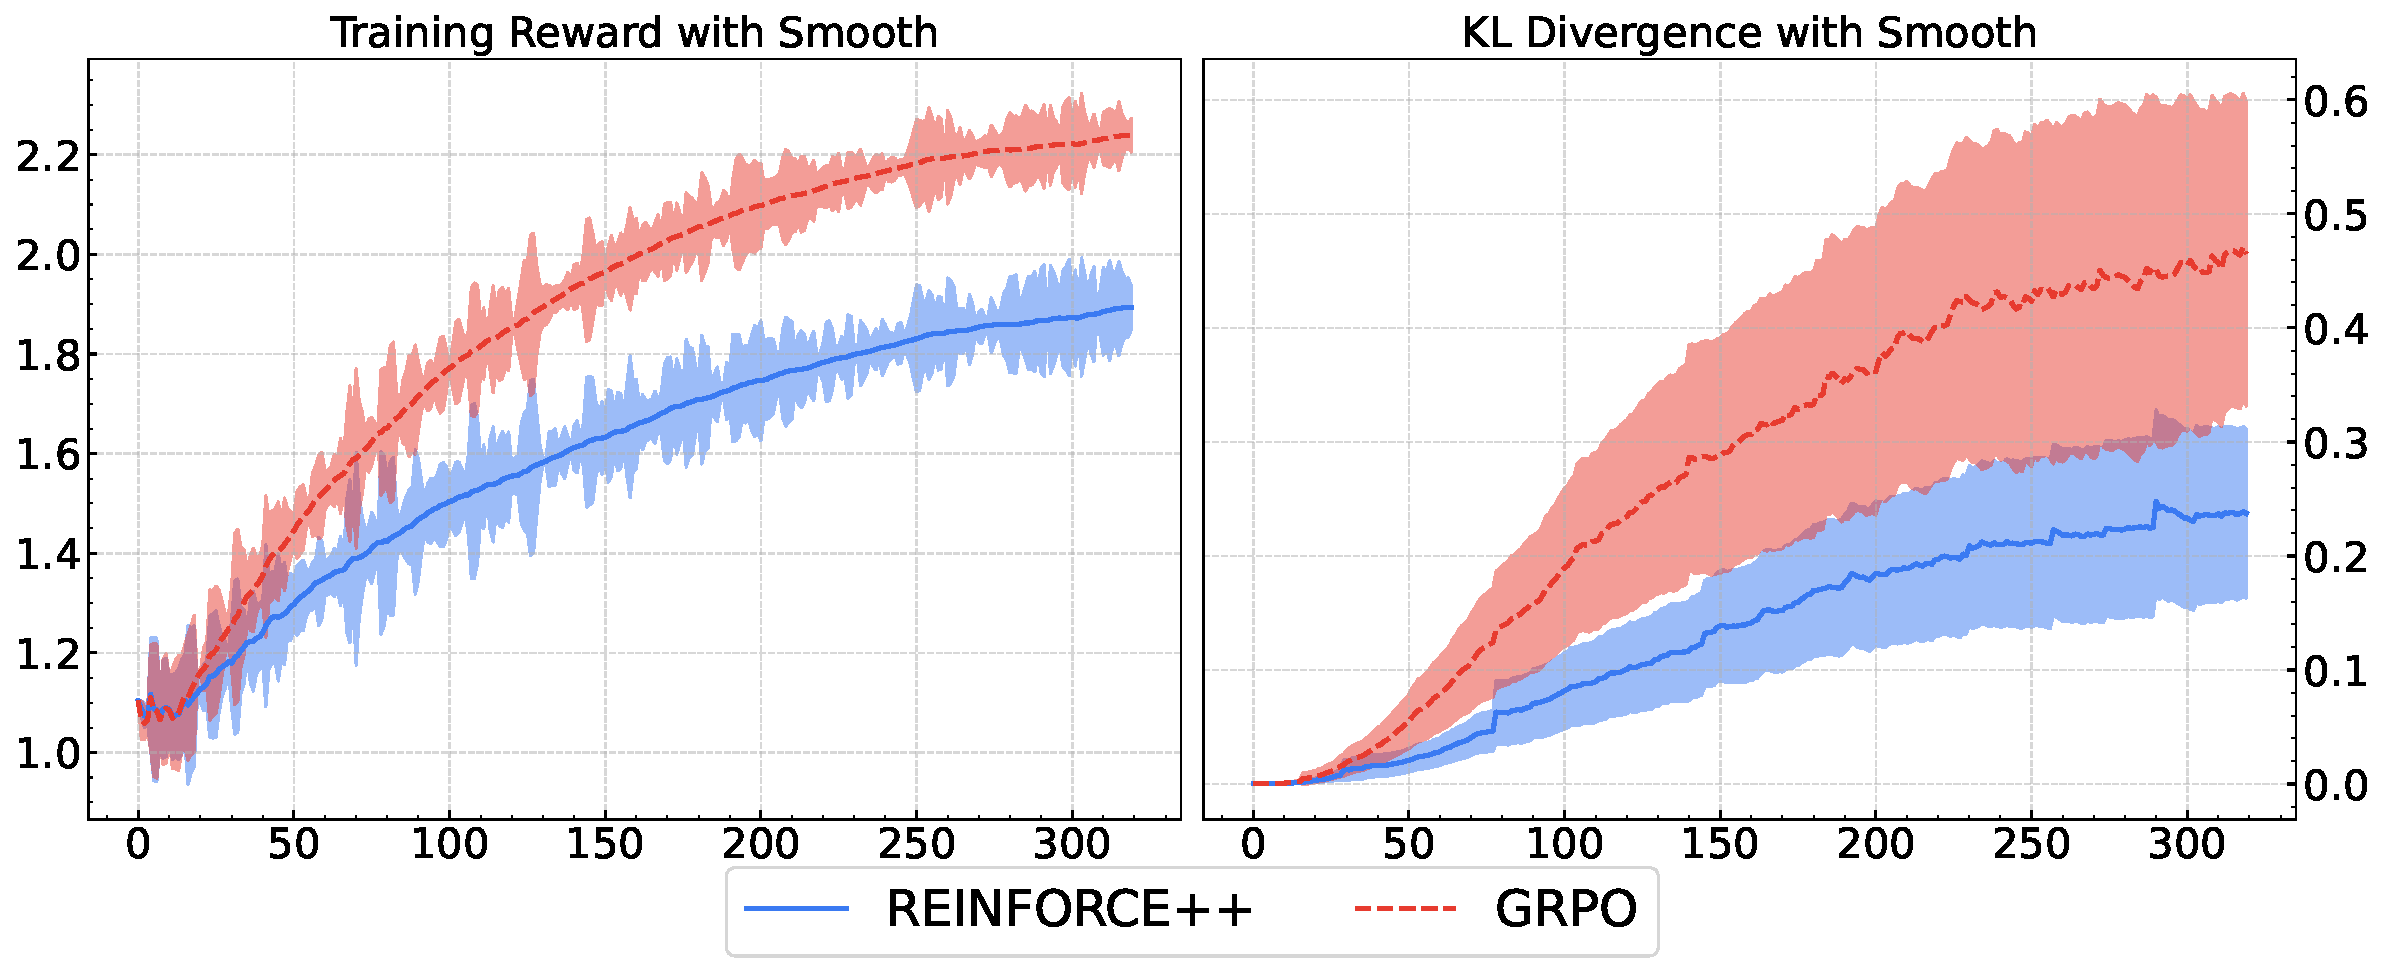
\includegraphics[width=0.9\linewidth]{imgs/orm_reward_kl.pdf}
    \caption{Comparison of smoothed Training Reward and KL Divergence. \ours ($k=1$) achieves strong rewards with significantly more stable (lower) KL divergence, avoiding GRPO's reward-hacking behavior.}
    \label{fig:orm_reward_kl}
\end{figure*}


\subsection{General RLHF}
First, we evaluate the \ours in its $k=1$ configuration, focusing on general-domain RLHF, where efficiency and prompt diversity are key.

\paragraph{Experimental Setup}
We use an instruction-following policy model (Llama-3-8B-SFT) and refine it using a Bradley-Terry reward model \citep{bai2022training} trained on $\sim$700K human preference pairs. The policy is trained on 20,000 diverse prompts. We compare \ours ($k=1$) with other critic-free methods: GRPO ($k=4$), RLOO ($k=4$), and ReMax ($k=1$ + 1).

\begin{table}[!htbp]
    \small
    \centering
    \begin{tabular}{l|cc|c}
    \toprule
                       & Score & Length  & Per Token    \\
    \midrule
    \textbf{\ours (k=1)} & 46.7        & 832   &  \textbf{0.0561} \\
    GRPO (k=4)         & \textbf{46.8} & 860       &  0.0544 \\
    RLOO (k=4)         & 44.6        & 866   &  0.0515 \\
    ReMax (k=1+1)      & 45.1        & \textbf{805}  &  0.0560 \\
    \bottomrule
    \end{tabular}
    \caption{Comparison on Chat-Arena-Hard \citep{li2024crowdsourced}. The single-sample \ours ($k=1$) achieves a top-tier score while being more token-efficient than the group-sampling GRPO.}
    \label{tab:general_exp}
\end{table}

\paragraph{Experimental Results}
As shown in \Cref{tab:general_exp}, the single-sample \textbf{\ours ($k=1$)} achieves a score of 46.7, statistically tied with the group-sampling GRPO (46.8). However, it produces shorter responses (832 tokens vs. 860), yielding a higher, more efficient per-token score (0.0561). This result indicates that for general tasks, group sampling ($k>1$) is unnecessary and may be suboptimal.

\paragraph{Results Analysis}
\Cref{fig:orm_reward_kl} shows the training dynamics. GRPO's reward rises quickly, but its KL divergence also increases rapidly, suggesting it is "hacking" the reward model. In contrast, \ours shows a more stable reward increase with a much smaller KL divergence. It highlights the stability of global normalization and its higher "KL-to-reward" conversion efficiency, avoiding the reward hacking seen in local normalization methods, which is often linked to length exploitation \citep{dubois2024length}.

% --- MODIFIED: This commented-out table was in the original file and removed by the user. Retaining its removal. ---
% \begin{table*}[!htbp]
%      \centering
%      \begin{tabular}{l|cccc|c}
%      \toprule
%                       & GSM8K  & MATH & HumanEval & MBPP    & Avg.        \\
%      \midrule
%      Base Model (before training) & 95.83 & 68.80 & 82.71 & 82.2 & 82.39 \\
%      \textbf{\ours (k=4)} & 96.21 & 75.20 & \textbf{85.98} & 84.39 &  \textbf{85.45} \\
%      % \varn (k=4) & 95.98  & 72.40 & 78.66 & \textbf{85.45} & 83.12 \\ % <-- MODIFIED: Removed this line per request
%      GRPO (k=4)         & 96.21  & 73.80 & 80.49 & 83.33 & 83.46 \\
%      RLOO (k=4)         & 96.44  & 72.40 & 79.27 & 82.54 & 82.67 \\
%      ReMax (k=1+1)      & \textbf{96.59}  & \textbf{75.40} & 78.66 & 82.54 & 84.05 \\
%      \bottomrule
%      \end{tabular}
%      \caption{Comparison on OOD benchmarks. The stable, \ours ($k=4$) achieves the best average OOD generalization.}
%      \label{tab:ood_exp}
% \end{table*}

% To confirm this, we evaluated OOD generalization on math and code tasks (\Cref{tab:ood_exp}). \ours ($k=4$) achieves the highest average OOD score (85.45), outperforming all other methods, including the group-sampling GRPO (83.46). It strongly supports our hypothesis: for general-domain RLHF, the stable, single-sample \ours provides the best generalization.
% --- END OF REMOVED SECTION ---


\subsection{Reasoning Experiments} % <-- MODIFIED: Changed heading to match user's logic
Next, we evaluate \ours (group-sample, $k>1$) in its target domain: complex reasoning, where group sampling is standard, and reward signals are often sparse (e.g., 0/1). We compare it directly with GRPO ($k > 1$).

\subsubsection{Long Reasoning Task}
We use rule-based rewards (RLVR) in mathematical reasoning settings \citep{guo2025deepseek,seed2025seed1}.

\paragraph{Analysis on Small-Scale Datasets}
To test for overfitting, we trained on only 30 questions from AIME-24 and evaluated on AIME-25. As shown in \Cref{tab:small_exp}, GRPO (local norm) achieves a near-perfect 95.0\% on the training set but completely fails on the test set (0.0 Pass@1), demonstrating catastrophic overfitting. In contrast, \ours with global norm, while scoring lower on the training set (71.0), shows significantly better generalization (2.5 Pass@1, 40.0 Pass@16). % <-- MODIFIED: User changed this from Baseline.

\begin{table}[!ht]
    \small
    \centering
    \begin{tabular}{l|ccc}
    \toprule
                       & AIME-24 (Train) & \multicolumn{2}{c}{AIME-25 (Test)} \\
    Pass@N             & N = 1  &  N = 1     &  N = 16 \\
    \midrule
    GRPO               & \textbf{95.0}   & 0.0        & 0.4 \\
    \textbf{\ours} & 71.0        & \textbf{2.5}& \textbf{40.0} \\ % <-- MODIFIED: User changed this from Baseline, I'm adding ($k>1$) for clarity
    \bottomrule
    \end{tabular}
    \caption{Comparison on a small training dataset. GRPO (local norm) overfits completely, while \ours (global norm) generalizes.}
    \label{tab:small_exp}
\end{table}


\Cref{fig:details} confirms this. GRPO (left) immediately overfits, mastering the training questions in just a few steps. \ours (right) learns more gradually, enabled by the stable global normalization signal. % <-- MODIFIED: User changed this from Baseline.

\begin{figure*}[!htbp]
    \centering
    \begin{subfigure}[b]{0.5\linewidth}
        \centering
        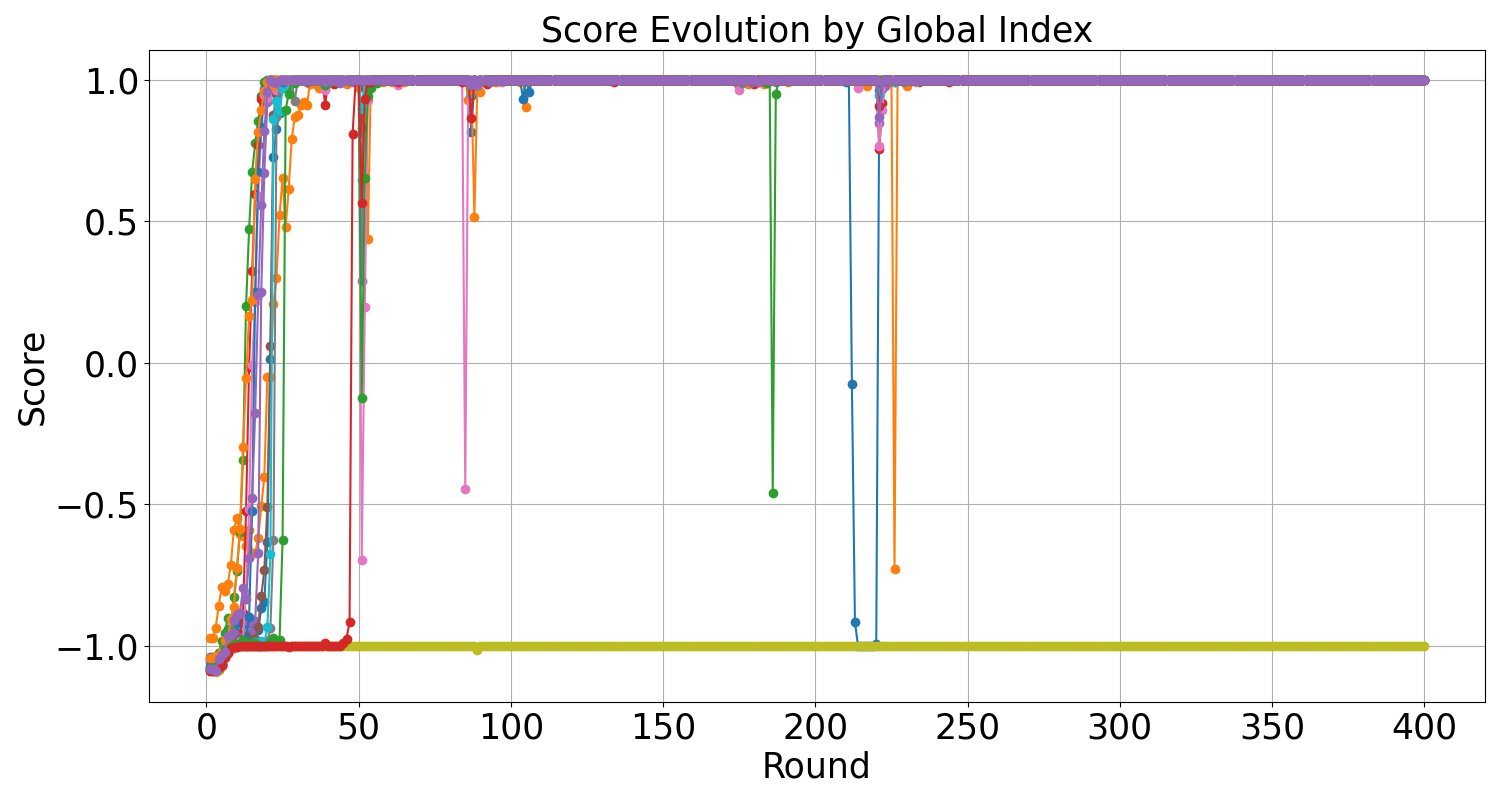
\includegraphics[width=\textwidth]{imgs/GRPO.png}
        % \caption{Lorem ipsum}
    \end{subfigure}%
    \hfill
    \begin{subfigure}[b]{0.5\linewidth}
        \centering
        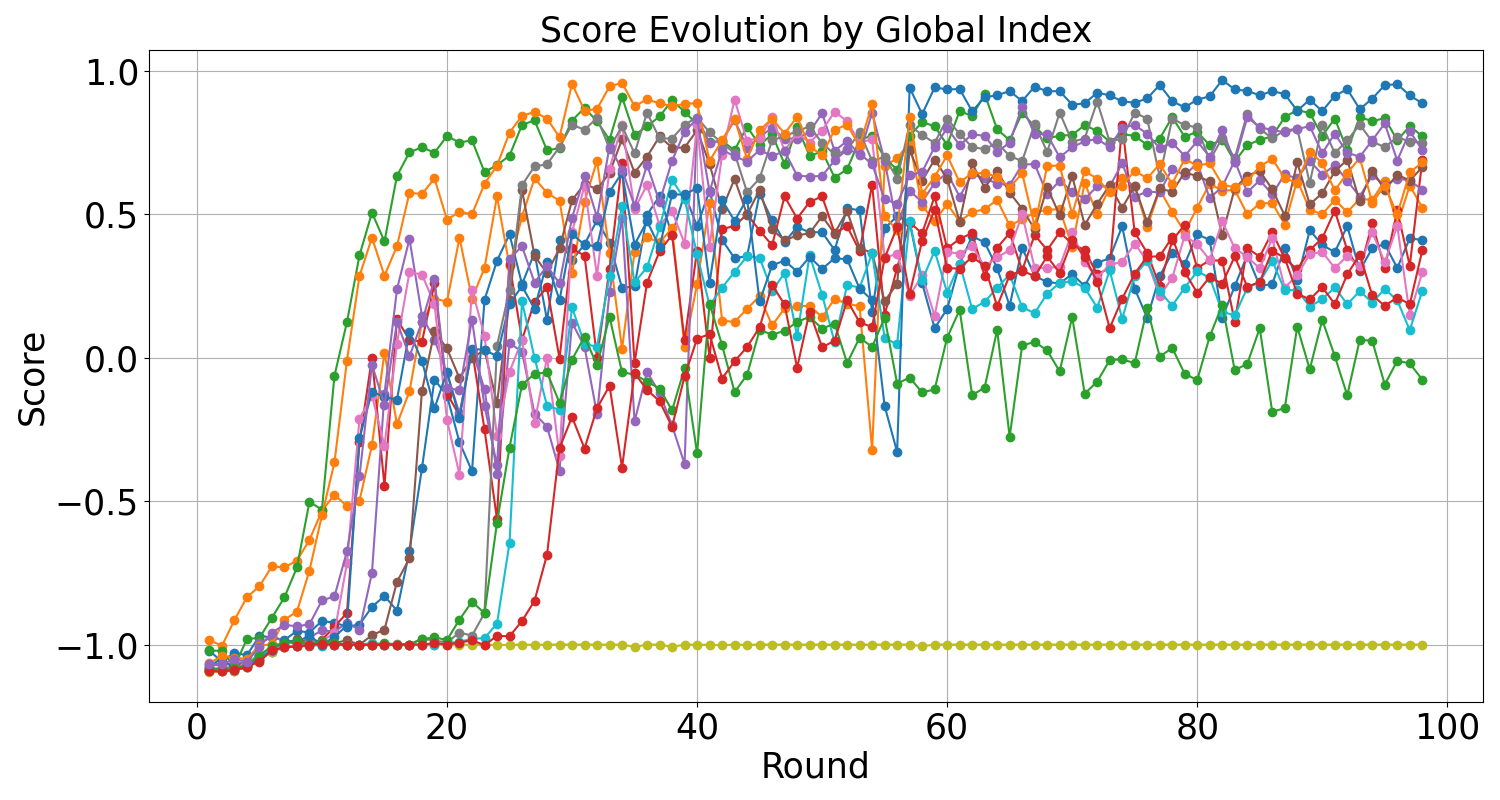
\includegraphics[width=\textwidth]{imgs/REINFORCE++.png}
    \end{subfigure}
    % --- MODIFIED: User changed this from Baseline. ---
    \caption{Training curves on a small prompt dataset. Left: GRPO (local norm) immediately overfits. Right: \ours (global norm) learns more stably.}
    \label{fig:details}
\end{figure*}

\paragraph{Logical Reasoning (K\&K Puzzles)}
We also tested on the Knights and Knaves (K\&K) puzzles \citep{xie2025logic, xie2024memorization}, where difficulty increases with the number of "people." \Cref{fig:logic_score} shows that while GRPO is competitive on easy tasks (2-3 people), its performance collapses on harder, OOD tasks (8 people). \ours is more robust, outperforming GRPO on all tasks with four or more people and achieving a much higher average score (62.1 vs. 55.7). % <-- MODIFIED: User changed this from Baseline.

\begin{figure}[!htbp]
    \centering
    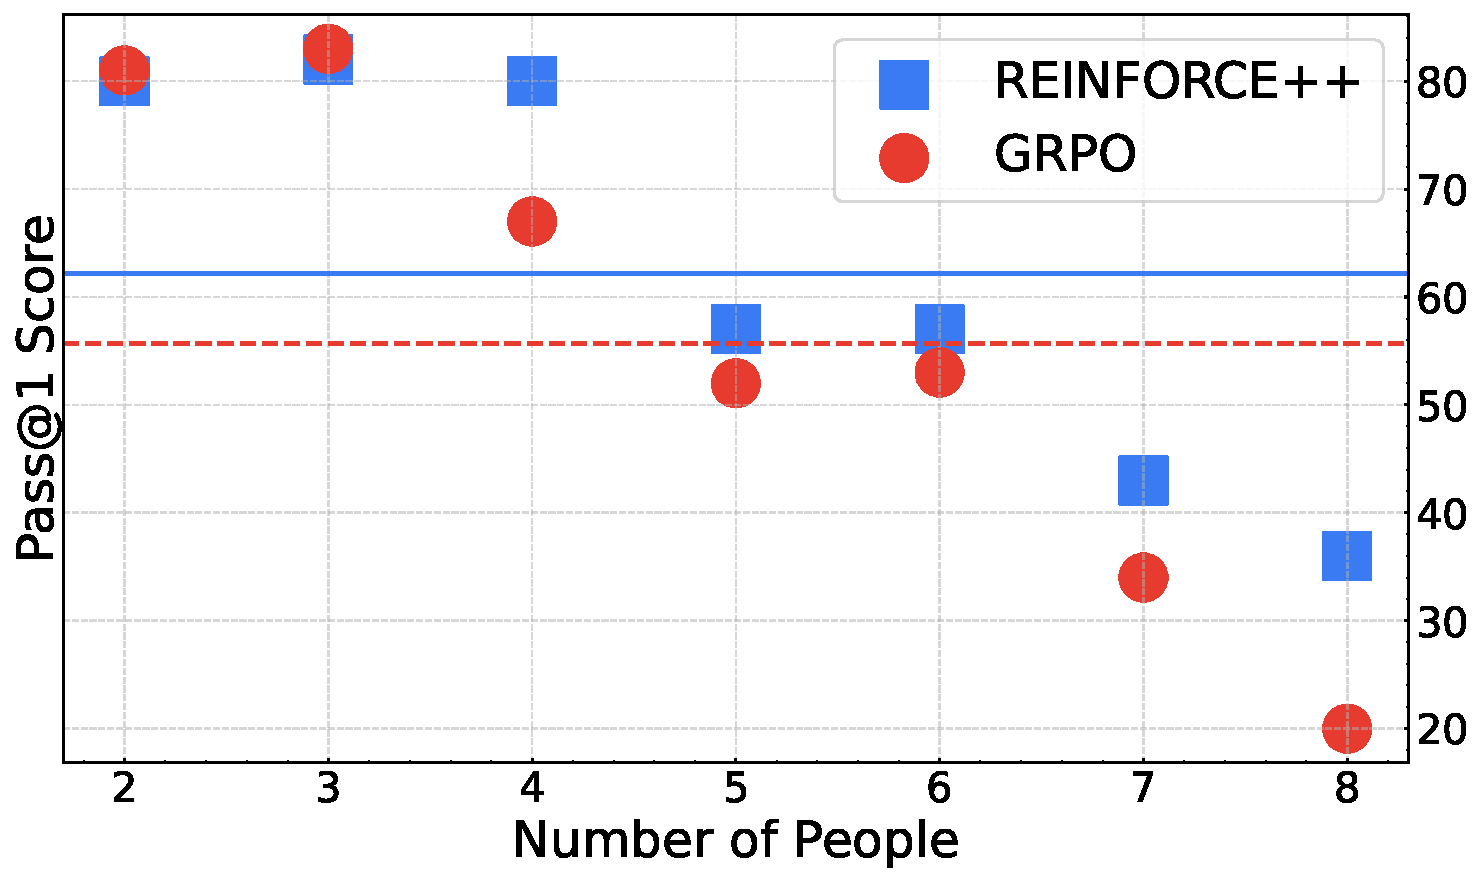
\includegraphics[width=0.7\linewidth]{imgs/logic_score.pdf}
    % --- MODIFIED: User changed this from Baseline. ---
    \caption{Comparison on logic benchmarks. \ours's global normalization provides better robustness to increasing task difficulty and OOD challenges (8 people).}
    \label{fig:logic_score}
\end{figure}


\paragraph{RL from Zero Setting}
Finally, we trained a Qwen2.5-Math-Base model from zero on MATH dataset splits \citep{guo2025deepseek}. \Cref{Tab:zero-experiment} shows that \ours again achieves better OOD generalization on the more challenging AIME-24 and AMC-23 datasets, while remaining competitive on the in-distribution MATH-500 test set. % <-- MODIFIED: User changed this from Baseline.

\begin{table*}[!htbp]
    \small
    \centering
    \begin{tabular}{l|ccc}
    \toprule
                       & AIME-24 (OOD) & AMC-23 (OOD) & MATH-500 (ID) \\
    Pass@N             & N = 8   &  N = 8   &  N = 1    \\
    \midrule
    GRPO               & 18.96       & 59.22    & \textbf{73.00}    \\
    \ours & \textbf{21.04}  & \textbf{60.47}   & 72.00     \\ % <-- MODIFIED: User changed this from Baseline.
    \bottomrule
    \end{tabular}
    % --- MODIFIED: User changed this from Baseline. ---
    \caption{Comparison on RL from Zero. \ours shows superior OOD performance.}
    \label{Tab:zero-experiment}
\end{table*}

% --- MODIFIED: This section was moved from the appendix by the user. It is a good change. ---
\subsection{Multi-step Reinforcement Learning}
Finally, to test performance in a complex, multi-step environment, we use the zero-shot agent setup from \cite{mai2025agent}, in which a Qwen 2.5 Base 7B model must learn to use Python tools to solve mathematical problems. It is a challenging scenario where group sampling ($k > 1$) and reward reshaping are crucial (see Appendix \Cref{appendix:best}).

\paragraph{Experimental Setup}
We adhere to the training and evaluation protocols of the ZeroTIR environment \cite{mai2025agent}. The backbone model is Qwen 2.5 Base 7B, trained using OpenRLHF \cite{hu2025open} with datasets from ORZ \cite{hu2024openrlhf} and DAPO \cite{yu2025dapo}. We assess performance on benchmarks including AIME 2024 \cite{aime2024card}, AIME-2025 \cite{aime2025card}, HMMT FEB-2024/2025, and CMIMC, using the \texttt{average@32} metric.

\paragraph{Experimental Result}
As shown in \Cref{tab:performance_comparison_main}, \varn achieves the highest average accuracy (24.10) across all benchmarks. It significantly outperforms both GRPO (22.58) and the full-critic PPO (21.85). It demonstrates that our stable, critic-free approach is highly effective for complex agentic tasks, surpassing even the heavyweight PPO algorithm. The combination of group-mean reshaping, stable global normalization, and the correct `k2` KL loss proves superior.

\begin{table*}[!htbp]
\small
\centering
\begin{tabular}{l|ccccc|c}
\toprule
\textbf{Algorithm} & AIME 24 & AIME 25 & HMMT 2025 & HMMT 2024 & CMIMC & \textbf{Avg} \\
\midrule
GRPO (local norm) & \textbf{31.66} & 21.87 & 16.97 & 17.70 & 24.68 & 22.58 \\
PPO (critic-based) & 30.20 & 21.66 & 15.00 & 18.43 & 23.95 & 21.85 \\
\textbf{RF++-Baseline (global norm)} & 30.83 & \textbf{27.18} & \textbf{17.91} & \textbf{18.95} & \textbf{25.62} & \textbf{24.10} \\
\bottomrule
\end{tabular}
\caption{Performance Comparison on complex tool-use benchmarks (average@32). \varn outperforms both GRPO (local norm) and PPO (critic-based) models.}
\label{tab:performance_comparison_main}
\end{table*}

\section{Best Practices} \label{appendix:best}

\subsection{General Principle}

This paper introduces two algorithms: \ours and \varn[n], with a key focus on selecting the appropriate algorithm based on task conditions.

Empirical evidence from the open-source community suggests that \varn[n] is particularly effective for sample filtering or more complex scenarios. For instance, in the multi-turn tool-calling setting, a high proportion of void (i.e., non-informative or incorrect) samples can destabilize training. In such cases, incorporating a baseline by subtracting the intra-group mean reward significantly improves training stability by effectively filtering out void samples. Moreover, this automatic reward reshaping reduces the need for designing complex reward structures. For example, \varn[n] supports both 0/1 and -1/1 reward schemes, while \ours performs best with symmetric rewards, such as -1/1 in RLVR tasks.

In contrast, for general-domain tasks where prompt diversity and efficiency are paramount, or for tasks where obtaining multiple reward signals for distinct responses is challenging—such as training with Process-Supervised Reward Models~(PRMs) or online real-time sampling—we recommend using \textbf{\ours ($k=1$)}. Our experiments (Section 4.1) show that it provides superior OOD generalization in these settings.

\subsection{Third-Party Validation}
The core principle of \ours, global advantage normalization, has been independently validated and adopted in several \textbf{subsequent} large-scale reasoning systems, confirming its stability and effectiveness.

\paragraph{LitePPO}~\citep{liu2025part}, which effectively combines \varn with a token-level loss, conducted experiments demonstrating that the global standard deviation is superior to the local standard deviation used in GRPO. Their results indicate more stable training and better generalization, which aligns with our findings.

\paragraph{ScaleRL}~\citep{khatri2025art} performed a detailed ablation study on advantage estimation methods in large-scale (16,000 GPU-hour) experiments. They directly compared batch-level normalization in \ours with prompt-level normalization in GRPO. Their findings concluded that batch-level normalization was "slightly superior in both compute efficiency and final performance," confirming the advantages of global normalization at scale.

\paragraph{DLER}~\citep{liu2025dler} found that when using truncation to control the output length of an LLM, batch-wise (global) normalization remains stable while group-wise (local) normalization shows declining accuracy. The study provides further evidence that global normalization is more robust to variations in training conditions and reward landscapes.

\section{Conclusion}\label{sec:conclusion}
In this paper, we present \ours, a critic-free RLHF framework designed to enhance training stability by addressing fundamental flaws in existing methods. We identified that prior critic-free algorithms, such as GRPO, rely on \textit{prompt-level (local)} advantage normalization, which we prove to be theoretically biased (Appendix \Cref{appendix:proof_GRPO}) and demonstrate to be practically unstable.

Our solution, \textbf{Global Advantage Normalization}, normalizes advantages across the entire batch, providing a stable and \textit{effectively unbiased} estimator (whose bias vanishes as batch size increases). We proposed two variants tailored for different needs:
\begin{enumerate}
    % --- MODIFIED: Conclusion updated to match the k>=1 logic ---
    \item \ours: For general-domain RLHF, we show the single-sample ($k=1$) approach is highly efficient and achieves superior OOD generalization. We also show that its application with $k>1$ is robust for reasoning tasks (Section 4.2).
    % --- END OF MODIFICATION ---
    \item \varn: For complex reasoning and agent tasks, this variant combines group-mean reshaping with stable global normalization and a theoretically sound $k_2$ estimator for KL.
\end{enumerate}

Our empirical results, supported by independent validation from multiple third-party systems, confirmed the effectiveness of this specialized approach. \ours demonstrated state-of-the-art generalization in general RLHF. \varn showed dramatic improvements in stability, preventing overfitting in low-data regimes and outperforming both GRPO and full-critic PPO in complex, long-horizon tool-use tasks. This work demonstrates that a theoretically sound, stable approach without a critic model can be more efficient and effective than traditional PPO.



\section*{AI Use Statement}

Generative AI tools assisted with manuscript preparation, including formatting, mathematical exposition, and proof revision. Experimental data and results were produced by the authors. The authors reviewed the AI-assisted content and take responsibility for the final manuscript and its accompanying artifacts.

\section*{Ethics Statement}

Reinforcement learning is increasingly used to steer large language models by optimizing them against a reward signal, including verifiable, programmatic rewards (RLVR) for domains such as math, code, and tool use. The main potential positive impact of this line of work is improved scalability and reproducibility of post-training: verifiable rewards can reduce reliance on human labeling and make optimization targets easier to audit and replicate. The critic-free methods studied here aim to support this use of reinforcement learning through shared advantage scaling and prompt-specific reward centering. Potential risks include reward gaming when verifiers are incomplete or mis-specified, and dual-use concerns if improved tool-use or problem-solving capabilities are deployed without safeguards. We recommend evaluating beyond verifier scores (e.g., robustness and red-teaming), stress-testing verifiers for exploitability, and using conservative deployment controls (e.g., access restrictions and monitoring) for systems trained with RL.

\section*{Reproducibility Statement}
Section~\ref{sec:method} specifies the algorithms, and Section~\ref{sec:experiment} describes the experimental settings. Appendix~\ref{appendix:batch_mean} specifies the response-wise loss reduction of the policy objective. Appendices~\ref{appendix:proof_GRPO} and~\ref{appendix:kl_design} provide assumptions and derivations for normalization and KL regularization.

\bibliography{reference}
\bibliographystyle{iclr2027_conference}

%%%%%%%%%%%%%%%%%%%%%%%%%%%%%%%%%%%%%%%%%%%%%%%%%%%%%%%%%%%%%%%%%%%%%%%%%%%%%%%
%%%%%%%%%%%%%%%%%%%%%%%%%%%%%%%%%%%%%%%%%%%%%%%%%%%%%%%%%%%%%%%%%%%%%%%%%%%%%%%
% APPENDIX
%%%%%%%%%%%%%%%%%%%%%%%%%%%%%%%%%%%%%%%%%%%%%%%%%%%%%%%%%%%%%%%%%%%%%%%%%%%%%%%
%%%%%%%%%%%%%%%%%%%%%%%%%%%%%%%%%%%%%%%%%%%%%%%%%%%%%%%%%%%%%%%%%%%%%%%%%%%%%%%
\appendix

\begin{center}
    {\Large \bfseries Appendix}
\end{center}

\section{Proof: The GRPO Advantage Estimator is Biased} \label{appendix:proof_GRPO}

\subsection{Assumptions and Settings}
We observe \(N\) rewards \(r_i\) for a prompt, and assume the true baseline is \(\theta\), such that
\[
r_i = \theta + \epsilon_i, \quad \epsilon_i \sim \mathcal{N}(0, \sigma^2),\quad i=1,\dots,N,
\]
with all advantage value \(\epsilon_i\) independent. Define
\[
\bar\epsilon = \frac{1}{N} \sum_{j=1}^N \epsilon_j, \quad
D = \sqrt{ \frac{1}{N} \sum_{j=1}^N (\epsilon_j - \bar\epsilon)^2 }, \quad
A_i = \frac{ \epsilon_i - \bar\epsilon }{D }.
\]
We will prove the following:

\begin{theorem}
For any finite \(N \ge 2\), the advantage estimator \(A_i\) is biased:
\[
\mathbb{E}[A_i \mid \epsilon_i] \ne \epsilon_i.
\]
\end{theorem}

\begin{proof}
We can prove our findings with the following steps:\\
\textbf{Step 1: Numerator Bias}
We rewrite the numerator:
\[
\epsilon_i - \bar\epsilon = \left(1 - \frac{1}{N} \right) \epsilon_i - \frac{1}{N} \sum_{j \ne i} \epsilon_j.
\]
Since the \(\epsilon_j\) for \(j \ne i\) are zero-mean and independent of \(\epsilon_i\),
\[
\mathbb{E}[\epsilon_i - \bar\epsilon \mid \epsilon_i] = \left(1 - \frac{1}{N} \right) \epsilon_i.
\]

\textbf{Step 2: Denominator Depends on \(\epsilon_i\)}

\textit{(a) Compute \(\mathbb{E}[D^2 \mid \epsilon_i]\):}
By definition,
\[
D^2 = \frac{1}{N} \sum_{j=1}^N (\epsilon_j - \bar\epsilon)^2 = \frac{1}{N} \sum_{j=1}^N \epsilon_j^2 - \bar\epsilon^2.
\]
Since
\[
\bar\epsilon = \frac{1}{N} \left( \epsilon_i + \sum_{j \ne i} \epsilon_j \right),
\]
and conditioning on \(\epsilon_i\) keeps the \(\epsilon_j\), \(j \ne i\), i.i.d.\ \(\mathcal{N}(0, \sigma^2)\), we obtain:
\[
\mathbb{E} \left[ \sum_{j=1}^N \epsilon_j^2 \mid \epsilon_i \right] = \epsilon_i^2 + (N-1) \sigma^2,
\]
\begin{align*}
\mathbb{E}[\bar\epsilon^2 \mid \epsilon_i]
&= \frac{1}{N^2} \mathbb{E} \left[ \left( \epsilon_i + \sum_{j \ne i} \epsilon_j \right)^2 \Big| \epsilon_i \right] \\
&= \frac{1}{N^2} \left( \epsilon_i^2 + 2 \epsilon_i \cdot \underbrace{\mathbb{E}\left[ \sum_{j \ne i} \epsilon_j \right]}_{0} + \mathbb{E} \left[ \left( \sum_{j \ne i} \epsilon_j \right)^2 \right] \right) \\
&= \frac{\epsilon_i^2 + (N-1) \sigma^2}{N^2}.
\end{align*}
Subtracting:
\begin{align}
\mathbb{E}[D^2 \mid \epsilon_i]
&= \frac{1}{N} (\epsilon_i^2 + (N-1) \sigma^2) - \frac{\epsilon_i^2 + (N-1)\sigma^2}{N^2} \nonumber \\
&= \underbrace{\frac{(N-1)^2}{N^2} \sigma^2}_{\alpha} + \underbrace{\frac{N-1}{N^2}}_{\beta} \epsilon_i^2 = \alpha + \beta \epsilon_i^2.
\label{eq:condD2}
\end{align}

\textit{(b) \(g(\epsilon_i)\) is Not Constant:}
Let \(g(\epsilon_i) = \mathbb{E}\left[1/D \mid \epsilon_i \right]\) and \(\mu(\epsilon_i) = \mathbb{E}[D^2 \mid \epsilon_i] = \alpha + \beta \epsilon_i^2\).

Using Taylor expansion of \(f(x) = 1/\sqrt{x}\) around \(x_0 = \mu(\epsilon_i)\):
\[
f(x) = \frac{1}{\sqrt{x_0}} - \frac{1}{2} \frac{x-x_0}{x_0^{3/2}} + \frac{3}{8} \frac{(x-x_0)^2}{x_0^{5/2}} + O((x-x_0)^3)
\]

Taking the conditional expectation:
\[
\begin{aligned}
g(\epsilon_i) 
&= \mathbb{E}[1/D \mid \epsilon_i] 
= \mathbb{E}\left[\frac{1}{\sqrt{D^2}} \mid \epsilon_i\right] 
= \mathbb{E}\left[f(D^2) \mid \epsilon_i\right], \quad \text{where } f(x) = \frac{1}{\sqrt{x}} \\
&\approx f(\mu(\epsilon_i)) + f'(\mu(\epsilon_i)) \cdot \mathbb{E}[D^2 - \mu(\epsilon_i) \mid \epsilon_i] + \frac{f''(\mu(\epsilon_i))}{2} \cdot \mathbb{E}[(D^2 - \mu(\epsilon_i))^2 \mid \epsilon_i] \\
&= \frac{1}{\sqrt{\mu(\epsilon_i)}} 
- \frac{1}{2 \mu(\epsilon_i)^{3/2}} \cdot \underbrace{\mathbb{E}[D^2 - \mu(\epsilon_i) \mid \epsilon_i]}_{=\,0} 
+ \frac{3}{8 \mu(\epsilon_i)^{5/2}} \cdot \text{Var}(D^2 \mid \epsilon_i) \\
&= \frac{1}{\sqrt{\mu(\epsilon_i)}} + \frac{3}{8} \cdot \frac{\text{Var}(D^2 \mid \epsilon_i)}{\mu(\epsilon_i)^{5/2}}
\end{aligned}
\]

Since \(\mu(\epsilon_i) = \alpha + \beta \epsilon_i^2\) with \(\beta > 0\), the first term alone shows that \(g(\epsilon_i)\) depends on \(\epsilon_i^2\) and hence is not constant.

\textbf{Step 3: Putting It Together}
Decomposing \(A_i\),
\[
A_i = \frac{\epsilon_i - \bar\epsilon}{D} = \left(1 - \frac{1}{N} \right) \frac{\epsilon_i}{D} - \left( \frac{1}{N} \sum_{j \ne i} \epsilon_j \right) \cdot \frac{1}{D}.
\]
For fixed \(\epsilon_i\), the conditional distribution of \(\sum_{j \ne i} \epsilon_j\) is symmetric about zero, while \(1/D\) is always positive. Thus:
\[
\mathbb{E} \left[ \left( \frac{-1}{N} \sum_{j \ne i} \epsilon_j \right) \cdot \frac{1}{D} \Big| \epsilon_i \right] = 0.
\]
It follows that
\[
\mathbb{E}[A_i \mid \epsilon_i] = \left(1 - \frac{1}{N} \right) \epsilon_i \cdot \mathbb{E} \left[ \frac{1}{D} \mid \epsilon_i \right] = \left(1 - \frac{1}{N} \right) \epsilon_i \cdot g(\epsilon_i).
\]

\textbf{Step 4: Concluding the Bias}
If \(A_i\) were unbiased, we would have:
\[
\left(1 - \frac{1}{N} \right) g(\epsilon_i) \equiv 1 \quad \Rightarrow \quad g(\epsilon_i) \equiv \frac{N}{N-1},
\]
which contradicts Step 2. Therefore, for any finite \(N \ge 2\),
\[
\mathbb{E}[A_i \mid \epsilon_i] \ne \epsilon_i.
\]
Hence \(A_i\) is a biased estimator.

\end{proof}

\section{KL Penalty Design}\label{appendix:kl_design}

In non-critic algorithms like \varn, a KL divergence term is often added as a separate loss to constrain the policy $\pi_{\theta}$ from deviating too far from a reference policy $\pi_{ref}$. In practice, this expectation is estimated using samples, and three familiar estimators are used.

Given the importance ratio $\delta(y) = \pi_{ref}(y|\cdot) / \pi_{\theta}(y|\cdot)$ (where $\pi_{\theta}$ is the sampling policy and $\pi_{ref}$ is the reference):
\begin{itemize}
    \item $k_{1}(y) = -\log \delta(y) = \log \frac{\pi_{\theta}(y|\cdot)}{\pi_{ref}(y|\cdot)}$
    \item $k_{2}(y) = \frac{1}{2}(\log \delta(y))^{2} = \frac{1}{2}\left(\log \frac{\pi_{ref}(y|\cdot)}{\pi_{\theta}(y|\cdot)}\right)^{2}$
    \item $k_{3}(y) = \delta(y) - 1 - \log \delta(y)$
\end{itemize}

We analyze which of these (k1, $k_2$, or $k_3$) is the correct choice when used as a separate loss term.

\paragraph{Theoretical Reverse KL Gradient}
We are training with samples from $\pi_{\theta}$, so we are approximating the **Reverse KL (RKL)**, $D_{KL}(\pi_{\theta}||\pi_{ref})$. The practical policy gradient for RKL is (more details are in \citep{liu2025rethinking}):
$$
\nabla_{\theta}\mathcal{J}_{RKL}(\theta) = \mathbb{E}_{y\sim\pi_{\theta}(\cdot|x)}\left[\left(\log\frac{\pi_{\theta}(y|x)}{\pi_{ref}(y|x)}\right)\nabla_{\theta}\log \pi_{\theta}(y|x)\right]
$$

\paragraph{k1 Analysis}
We can **exclude k1** as a loss term. Its gradient does not depend on $\pi_{ref}$ and thus provides no constraining effect. The loss $\mathcal{J}_{k{1}} = \mathbb{E}_{y\sim\pi_{\theta}}[\log \pi_{\theta} - \log \pi_{ref}]$ differentiates to $\nabla_{\theta}\mathcal{J}_{k{1}} = \mathbb{E}_{y\sim\pi_{\theta}}[\nabla_{\theta}\log \pi_{\theta}]$, as the $\pi_{ref}$ term vanishes. (Note: k1 *is* used inside the reward for REINFORCE++, but not as a separate loss term).

\paragraph{$k_2$ Analysis}
The $k_2$ estimator provides a gradient that is **equivalent to the theoretical Reverse KL gradient**.

The $k_2$ loss is (noting that $(\log \frac{\pi_{\theta}}{\pi_{ref}})^2 = (\log \frac{\pi_{ref}}{\pi_{\theta}})^2$):
$$
\mathcal{J}_{k{2}as~loss}(\theta)=\mathbb{E}_{y\sim\pi_{\theta}(\cdot|x)}\left[\frac{1}{2}\left(\log\frac{\pi_{\theta}(y|x)}{\pi_{ref}(y|x)}\right)^{2}\right]
$$
Differentiating the term inside the expectation gives:
\begin{align*}
\nabla_{\theta}\left[\frac{1}{2}\left(\log\frac{\pi_{\theta}}{\pi_{ref}}\right)^{2}\right] &= \left(\log\frac{\pi_{\theta}}{\pi_{ref}}\right) \cdot \nabla_{\theta}\left(\log\frac{\pi_{\theta}}{\pi_{ref}}\right) \\
&= \left(\log\frac{\pi_{\theta}}{\pi_{ref}}\right) \cdot \nabla_{\theta}(\log \pi_{\theta} - \log \pi_{ref}) \\
&= \left(\log\frac{\pi_{\theta}}{\pi_{ref}}\right)\nabla_{\theta}\log \pi_{\theta}
\end{align*}
When we take the expectation over $y \sim \pi_{\theta}$, the gradient of the $k_2$ loss becomes:
$$
\mathbb{E}_{y\sim\pi_{\theta}}\left[\left(\log\frac{\pi_{\theta}(y|x)}{\pi_{ref}(y|x)}\right)\nabla_{\theta}\log \pi_{\theta}(y|x)\right]
$$
This \emph{perfectly matches} the practical RKL gradient. Therefore, $k_2$ is the theoretically correct and stable choice.

\paragraph{$k_3$ Analysis}
The $k_3$ gradient is problematic. It is theoretically an estimator for the **Forward KL** ($KL(\pi_{ref}||\pi_{\theta})$), not the Reverse KL. There is a mismatch: we are sampling from $\pi_{\theta}$, but the Forward KL gradient requires sampling from $\pi_{ref}$.

This method, used in GRPO, suffers from two major issues:
\begin{itemize}
    \item \textbf{Extremely High Variance:} When $\pi_{\theta}(y)$ becomes tiny for a sample $y$ where $\pi_{ref}(y)$ is moderate, the importance weight $\frac{\pi_{ref}(y)}{\pi_{\theta}(y)}$ in the gradient estimator explodes, leading to "infinite variance".
    \item \textbf{Numerical Instability:} It requires computing $p/q$ via $\exp(\log p - \log q)$, which is prone to overflow.
\end{itemize}
The result explains why methods using $k$ require frequent resetting of $\pi_{ref}$ to prevent the policies from diverging and the $k_3$ estimator from becoming unstable.

\paragraph{Conclusion}
Based on this analysis, the $k_2$ estimator is the optimal choice for the KL loss term, as it accurately and stably estimates the Reverse KL gradient. We therefore use the $k_2$ estimator in our \varn algorithm.
% --- END OF MODIFIED SECTION ---

%%%%%%%%%%%%%%%%%%%%%%%%%%%%%%%%%%%%%%%%%%%%%%%%%%%%%%%%%%%%%%%%%%%%%%%%%%%%%%%
%%%%%%%%%%%%%%%%%%%%%%%%%%%%%%%%%%%%%%%%%%%%%%%%%%%%%%%%%%%%%%%%%%%%%%%%%%%%%%%

\end{document}

% This document was modified from the file originally made available by
% Pat Langley and Andrea Danyluk for ICML-2K. This version was created
% by Iain Murray in 2018, and modified by Alexandre Bouchard in
% 2019 and 2021 and by Csaba Szepesvari, Gang Niu and Sivan Sabato in 2022.
% Modified again in 2023 and 2024 by Sivan Sabato and Jonathan Scarlett.
% Previous contributors include Dan Roy, Lise Getoor and Tobias
% Scheffer, which was slightly modified from the 2010 version by
% Thorsten Joachims & Johannes Fuernkranz, slightly modified from the
% 2009 version by Kiri Wagstaff and Sam Roweis's 2008 version, which is
% slightly modified from Prasad Tadepalli's 2007 version which is a
% lightly changed version of the previous year's version by Andrew
% Moore, which was in turn edited from those of Kristian Kersting and
% Codrina Lauth. Alex Smola contributed to the algorithmic style files.
